\section{Results}
\label{sec:results}

We evaluate the methods presented in a variety of scenes and compare their mean squared errors (MSE) with respect to time. The reference images were produced using a large number of samples with an unbiased unidirectional path tracer using light and BSDF MIS sampling to compute direct lighting. To ensure a fair comparison, the runtimes given include the maximum visible frustum pre-computation step.

\subsection*{Experiment 1}

\todo[inline]{The concrete experiments and comparisons to do are not finalized yet, so I cannot write about them in detail. subsections of this structure will be repeated for each of the experiment setups}

We first compare each method in {\color{red} x} scene(s) containing {\color{red} description of the properties of the scene(s)} (\autoref{fig:fake-results}). As demonstrated {\color{red} discussion of the results}

\begin{figure*}[p]
    \centering
    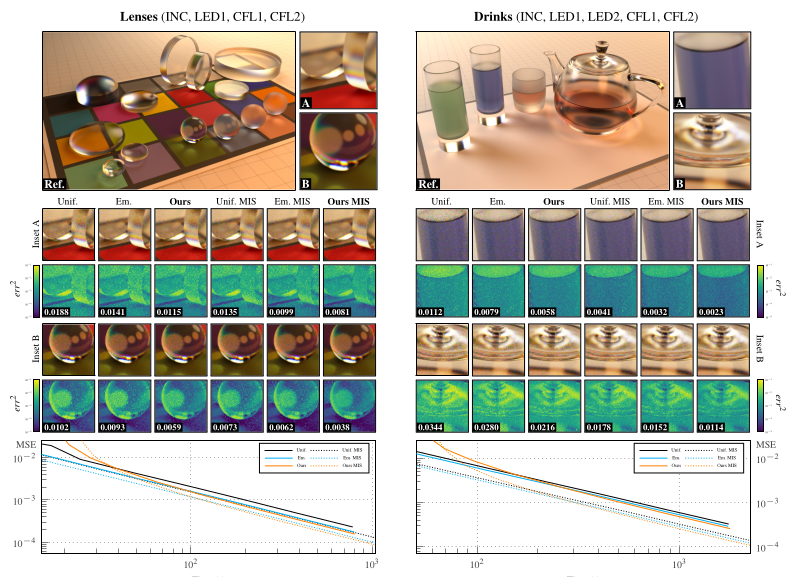
\includegraphics[width=0.95\textwidth]{mark-graph.png}
    \caption{{\color{red} (The results here are not mine!, Just a screenshot from one of Mark's papers to illustrate the general layout of the image)} 
    We compare the convergence rates for light sampling (Light), light-portal-projection (Proj) sampling, and light-portal MIS sampling (MIS) each method with and without frustum culling for a variety of scenes. The listed errors are for the highlighted image insets. As demonstrated, projection sampling generally is the most robust method, but converges slightly slower for scenes where the light is comparatively small in comparison to the portal}
    \label{fig:fake-results}
\end{figure*}